\LoadClass{NewTeX}
\documentclass{NewTeX}
\usepackage[utf8]{inputenc}
\usepackage{tabularx}
\usepackage{multirow}
\title{2SV317-BM: Projet -- Analyses exploratoires de données multivariées}
\author{Marion ROSEC, Evann DREUMONT}
\date{Décembre 2022}

\setmonofont{Fira Code Light}[
    Scale=0.8,
]

\usepackage{hyperref}
\usepackage{graphicx}
\usepackage{float}

\begin{document}

    \maketitle


    \section{Introduction}\label{sec:introduction}

    Dans cette étude, nous avons examiné le jeu de données \href{https://archive.ics.uci.edu/ml/datasets/SPECTF+Heart}{SPECTF Heart Data Set}, qui décrit le diagnostic de la perfusion myocardique à l'aide d'images de tomographie par émission monophotonique (ou SPECT, acronyme de l'anglais 'Single photon emission computed tomography') cardiaques.
    La tomographie par émission monophotonique est une technique de scintigraphie qui utilise un ensemble de caméras gamma tournant autour du patient pour produire des images et des reconstructions 3D des organes et de leur métabolisme.
    Le diagnostic de la perfusion myocardique est un examen de cardiologie nucléaire qui vise à évaluer l'apport sanguin au muscle cardiaque (myocarde).
    Le but de cet examen est de détecter la présence ou l'absence de coronaropathie, qui est une maladie des artères qui peut entraîner une ischémie myocardique, c'est-à-dire un apport sanguin insuffisant au muscle cardiaque.
    Le diagnostic de la perfusion myocardique est important car il permet de détecter les maladies cardiaques, telles que la coronaropathie, qui peuvent entraîner des complications graves si elles ne sont pas traitées à temps.
    Une analyse exploratoire de ces données pourrait permettre de développer de meilleurs modèles de diagnostic de la perfusion myocardique, ce qui pourrait améliorer la prise en charge des patients atteints de maladies cardiaques.
    En outre, une telle analyse pourrait également permettre de mieux comprendre les mécanismes sous-jacents à ces maladies et de développer de nouvelles stratégies de prévention et de traitement.
    En fin de compte, cela pourrait contribuer à améliorer la santé cardiaque globale et à réduire la morbidité et la mortalité liées aux maladies cardiaques.


    \section{Méthodologie}\label{sec:methodologie}

    Du fait le la complexité d'utilisé des données d'imagerie 3D en machines learning (que ce soit en taille, ou en puissance de calcul), la base de données de 267 ensembles d'images SPECT (patients) a été traitée pour extraire les caractéristiques qui résument les images SPECT originales.
    Les données sont donc résumées en 44 caractéristiques continues pour chacun des patients et sont de la forme :

    \begin{itemize}
        \item F$n$R : qui représente le nombre moyen de pixels après traitement de l'image localisé dans la zone d'intérêts $n$ au repos pour $n$ allant de 1 à 22.
        \item F$n$S : qui représente le nombre moyen de pixels après traitement de l'image localisé dans la zone d'intérêts $n$ dans des conditions de stress (effort) pour $n$ allant de 1 à 22.
    \end{itemize}

    Toutes ces variables sont des entiers allant de 0 à 100.
    Chacun des patients est classé en deux catégories : normal et anormal et un algorithme a été utilisé (CLIP3) pour prédire un diagnostic (colonne \verb|OVERALL_DIAGNOSIS| et donc en réalité, 45 attributs si nous prenons en compte cette colonne), nous savons également que cet algorithme avait une précision de 77\% par rapport aux diagnostics des cardiologistes.

    Lors de ce projet, nous avons pour des raisons de simplicité décider de n'utiliser que des classes et de n'avoir dans le notebooks réalisant l'analyse que des appels a des fonctions préalablement définies.
    Toujours dans un but d'avoir un code propre et compréhensible, nous avons choisi de nous inspirer de l'API utilisé dans le package \verb|sklearn| qui nous a été introduit au cours de ce cours.
    Nous avons alors défini deux classes abstraites qui se trouvent dans le dossier base, qui, bien que définissant une méthode qui sera hérité et deux méthodes abstraites, cette classe tend plus vers une interface que vers une classe abstraite et dans les faits, ici, nous avons plus affaire à une composition que de l'héritage classique, mais là n'est pas le sujet.
    Nous avons ainsi :
    \begin{itemize}
        \item La classe abstraite \verb|BaseTransformer|: la classe avec laquelle nous implémenterons les différentes méthodes qui nous permetterons de transformer nos données.
        Elle définit deux méthodes abstraites :
        \subitem \verb|fit|: qui calcule les paramètres nécessaires au modèle pour pouvoir ensuite transformer les données
        \subitem \verb|transform|: qui va alors transformer les données passées en paramètres en fonctions des paramètres calculer au préalable. \\
        Elle définit également une méthode \verb|fit_transform| qui va executer la méthode \verb|fit| et retourner le résultat de la méthode \verb|transform|.
        \item Et La classe abstraite \verb|BaseClassifier|: la classe avec laquelle nous hériterons lorsque nous implémenterons nos classifieurs.
        Elle définit deux méthodes abstraites :
        \subitem \verb|fit|: qui calcul les paramètres nécessaire au classifieur.
        \subitem \verb|predict|: qui associe classifie les données fournies en entrée, il faut donc au préalable avoir fait appel à la méthode \verb|fit| de la classe. \\
        Elle a défini également une méthode \verb|fit_predict| qui va executer la méthode \verb|fit| et retourner le résultat de la méthode \verb|predict|.
    \end{itemize}

    \begin{figure}[H]
        \centering
        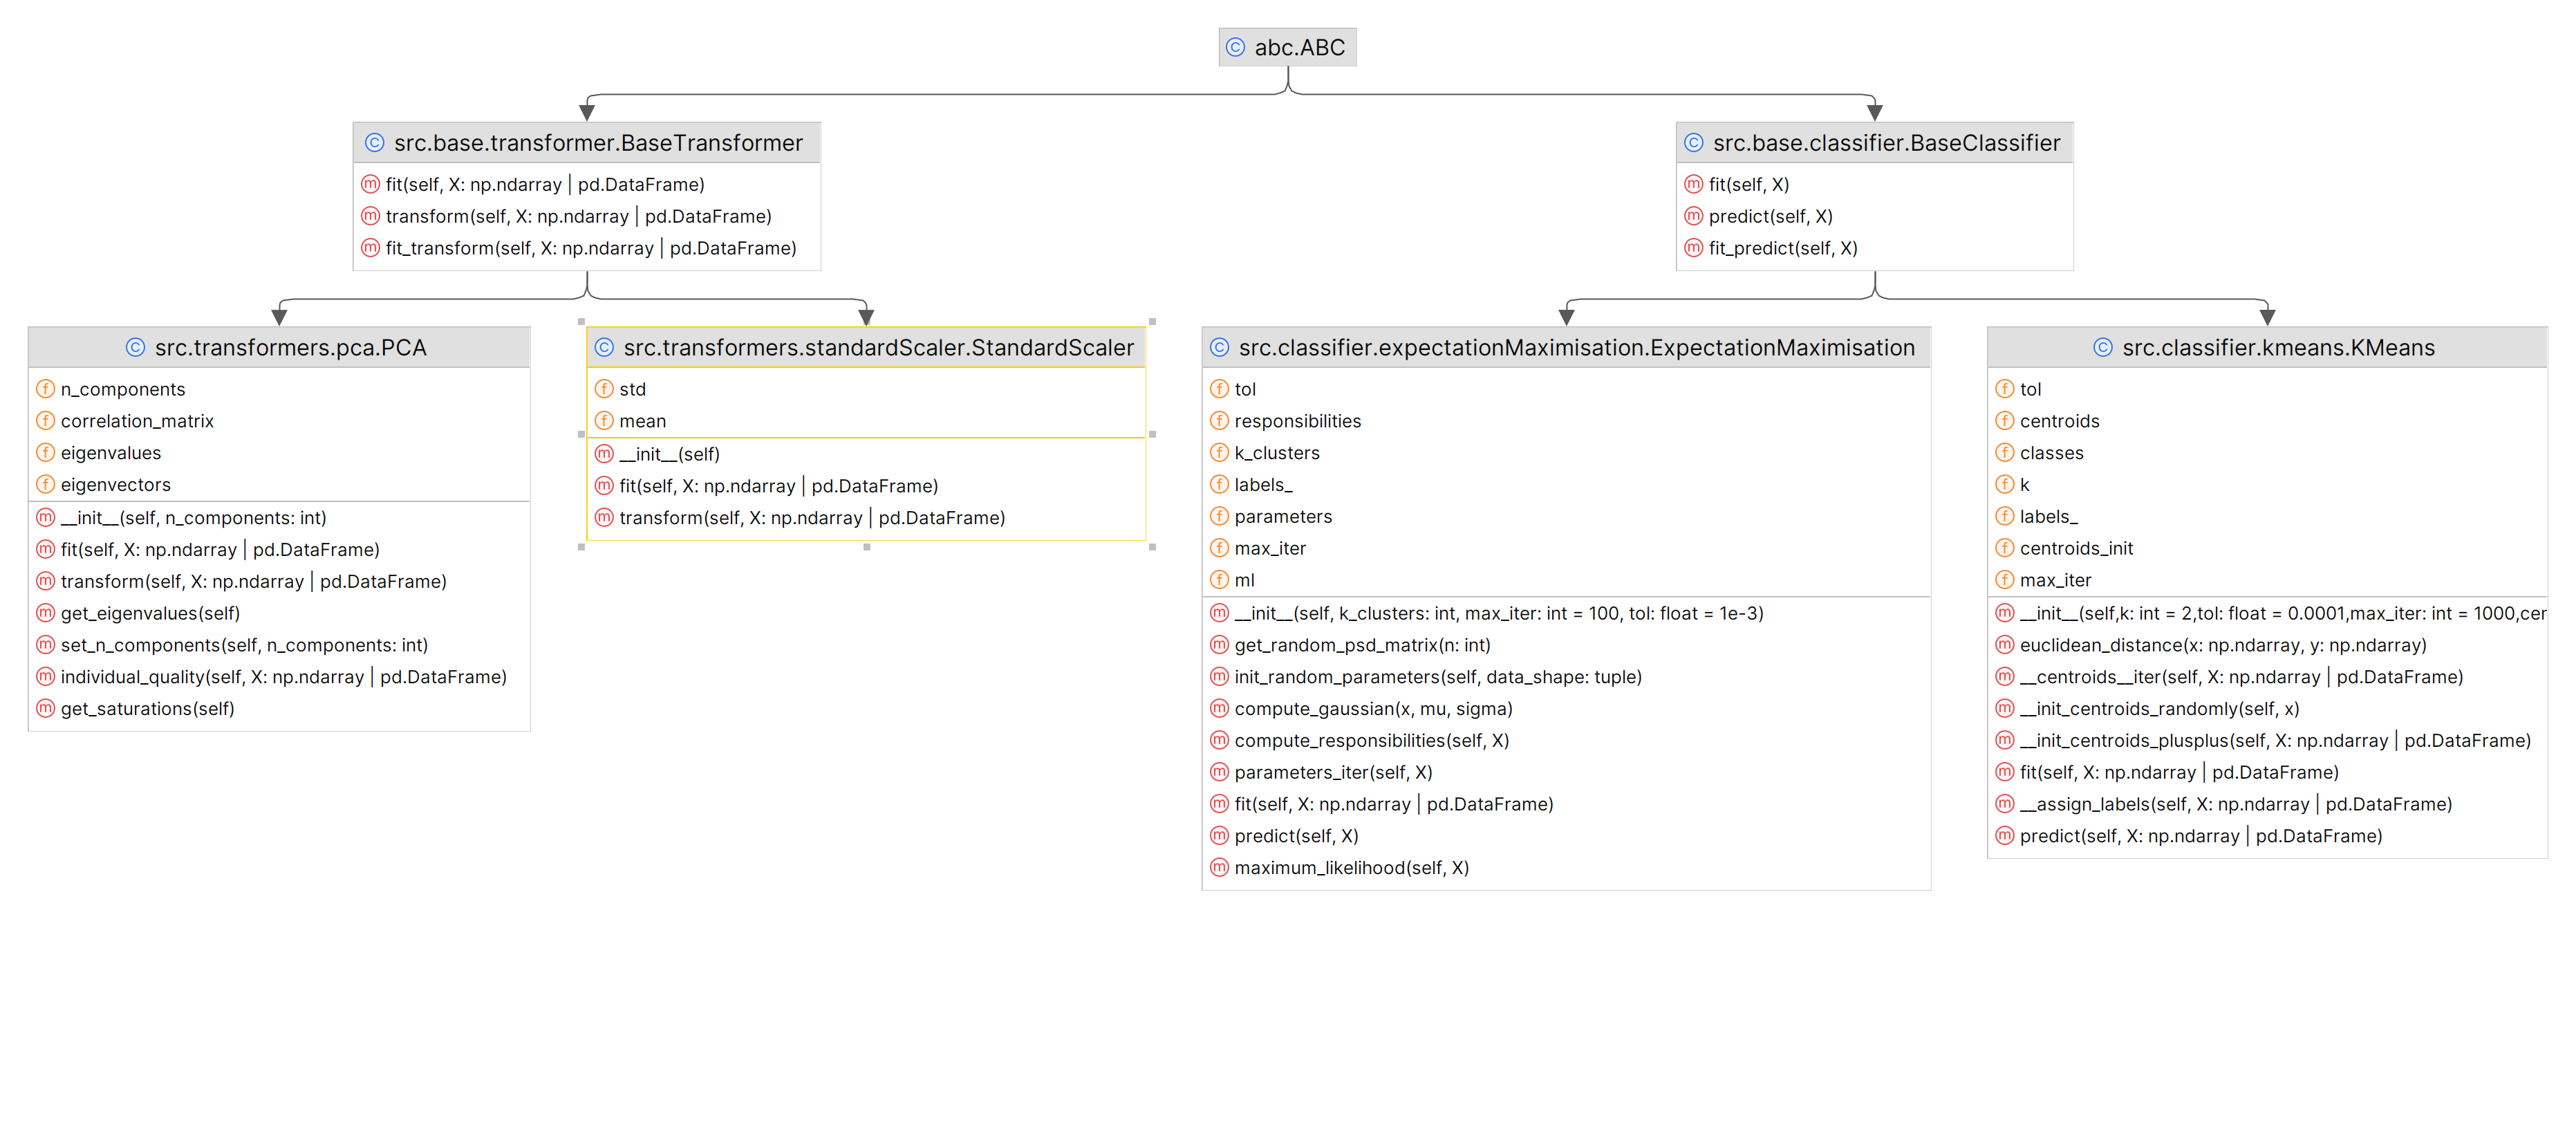
\includegraphics[scale=0.12]{./api_uml}
        \caption{UML}
        \label{fig:uml}
    \end{figure}

    Une fois ces deux classes implémentées, nous avons pu alors implémenter les autres classes qui découlent de celles-ci, donnent l'api (schématiser par la figure~\ref{fig:uml} ).

    \subsection{StandardScaler}\label{subsec:standardscaler}
    Dans un premier temps nous avons définis une nouvelle classe \verb|StandardScaler| qui hérite de \verb|BaseTransformer|.
    Son but est de normaliser les données, autrement dit de les centrer réduire.

    \subsection{PCA}\label{subsec:pca}
    Ensuite nous avons défini la classe PCA héritant de la classe \verb|BaseTransformer|, elle permet de réaliser une analyse en composante principale, c'est une méthode statistique utilisée en analyse de données qui permet de résumer l'information présente dans un jeu de donnée en réduisant le nombre de variables.
    Afin de faciliter l'usage de cette classe, nous avons mis en places différentes méthodes comme le setter \verb|set_n_conponents| qui permet de sélectionner le nombre de composantes voulu en sortie de la fonction \verb|transform| sans devoir instancier à nouveau une classe et appeler à nouveau la méthode fit de la classe (sachant que la méthode fit calculs les paramètres nécessaires à l'application de la méthode, à savoir ici, calculer les valeurs propres et les vecteurs propres de la matrice de corrélation).
    De même, nous avons défini différent getter qui permette de récupérer différents paramètres calculer comme les valeurs propres ou encore les saturations des axes, enfin nous avons également définis une méthode, \verb|individual_quality| permettant de récuper la qualité de chacun des points.

    \subsection{KMeans}\label{subsec:kmeans}
    Ici, nous avons affaire a la première classe qui n'est pas un transformer mais un classifier et qui donc hérite de la classe abstraitee \verb|BaseClassifier|.
    C'est une méthode de partitionnement des données, cherchant à optimiser la position de différents centroides (centre de cluster) en fonctions des données.
    Nous avons également implémenté l'algorithme d'initialisation k-means++, qui permet une initialisation plus intelligente des centroides améliorant la qualité du clustering, puisque l'algorithme est très sensible à l'initialisation.

    \subsection{ExpectationMaximisation}\label{subsec:expectationmaximisation}
    Enfin nous avons implémenter cette classe qui hérite de la classe abstraite \verb|BaseClassifier|.
    C'est l'implémentation d'un algorithme itératif permettant de trouver les paramètres de maximum de vraissemblance d'un modèle probabiliste.
    Ici le modèle probabiliste est un modèle de mélange gaussien, c'est-à-dire un mélange de différentes lois normales dans différente proportion dans le but de classifier les données, nous cherchons ainsi ici les paramètres de moyenne $\mu$, de variance $\sigma$ et proportion $\pi$ du mélange gaussien.
    Au cours de cette implémentation nous nous sommes trouvés face à différents problèmes, en effet : en fonctions de l'initialisation aléatoire, nous obtenions parfois l'intégralité des responsabilités égales a 0, ce qui entrainait une division par 0, de même parfois il est arrivé que les paramètres sigma ne soient plus des "positive semi-definite matrix" entrainant une exception lors de l'appelle de la méthode \verb|compute_gaussian|.
Malgré de nombreuses recherches ils nous a été impossible de trouver l'origine du problèmes, de plus sachant que parfois l'algorithme marchait bien, nous avons pu implémente une solution temporaire, a savoir que lorsque la fonction rencontrais l'une ou l'autre erreur, elle relancais entièrement la méthode \verb|fit|, avec donc, de nouveaux paramètres permettant alors d'obtenir des résultats et non pas s'arrêter sur une erreur. Néanmoins cette correction reste imparfait et une meilleurs implémentation serais nécessaires.


Ainsi maintenant que nous avons implémenter ces classes, nous pouvons alors réaliser notre analyse et essayer voir si une des méthodes automatiques nous permet de trouver des clusters satisfaisant pour une prédictions automatique par le futur.

\section{Résultats}\label{sec:resultats}




\section{Conclusion}\label{sec:conclusion}


\end{document}